%Copyright 2014 Jean-Philippe Eisenbarth
%This program is free software: you can 
%redistribute it and/or modify it under the terms of the GNU General Public 
%License as published by the Free Software Foundation, either version 3 of the 
%License, or (at your option) any later version.
%This program is distributed in the hope that it will be useful,but WITHOUT ANY 
%WARRANTY; without even the implied warranty of MERCHANTABILITY or FITNESS FOR A 
%PARTICULAR PURPOSE. See the GNU General Public License for more details.
%You should have received a copy of the GNU General Public License along with 
%this program.  If not, see <http://www.gnu.org/licenses/>.

%Based on the code of Yiannis Lazarides
%http://tex.stackexchange.com/questions/42602/software-requirements-specification-with-latex
%http://tex.stackexchange.com/users/963/yiannis-lazarides
%Also based on the template of Karl E. Wiegers t
%http://www.se.rit.edu/~emad/teaching/slides/srs_template_sep14.pdf
%http://karlwiegers.com

\documentclass{scrreprt}
\usepackage{graphicx}

\graphicspath{ {images/} }
\usepackage{url}
\usepackage{listings}
\usepackage{caption}
\usepackage{underscore}
\usepackage[bookmarks=true]{hyperref}
\usepackage[utf8]{inputenc}
\usepackage[english]{babel}
\usepackage{xcolor}
\usepackage{enumitem}
\usepackage{float}
\restylefloat{table}
\setlist{nosep}


\makeatletter
\newcommand\renewlistof[3]%
   {\renewcommand#1%
      {\section*{#3}%
       \addcontentsline{toc}{chapter}{#3}%
       \markboth{#3}{#3}%
       \@starttoc{#2}%
      }%
   }
\makeatother
\renewlistof\listoffigures{lof}{\listfigurename}
\renewlistof\listoftables{lot}{\listtablename}

\newcommand{\stimulus}[1] {
  \begin{enumerate}[leftmargin=5.7\parindent, label=Stimulus:]
  \item #1
  \end{enumerate}
  
  }
  \newcommand{\response}[1] {
  \smallskip
  \begin{enumerate}[leftmargin=6\parindent, label=Response:]
  \item #1
  \end{enumerate}
  }

\hypersetup{
    bookmarks=false,    % show bookmarks bar?
    pdftitle={Software Requirement Specification},    % title
    pdfauthor={Arif Ahmet Balik, Huseyin Bayraktar, Omer Can},                     % author
    pdfsubject={TeX and LaTeX},                        % subject of the document
    pdfkeywords={TeX, LaTeX, graphics, images}, % list of keywords
    colorlinks=true,       % false: boxed links; true: colored links
    linkcolor=blue,       % color of internal links
    citecolor=black,       % color of links to bibliography
    filecolor=black,        % color of file links
    urlcolor=purple,        % color of external links
    linktoc=page            % only page is linked
}%
\def\myversion{0.5}
\date{}
%\title
\usepackage{hyperref}
\begin{document}


\begin{flushright}
    \rule{16cm}{5pt}\vskip1cm
    \begin{bfseries}
        \Huge{SOFTWARE REQUIREMENTS\\ SPECIFICATION}\\
        \vspace{1.9cm}
        for\\
        \vspace{1.9cm}
        Student Attendance Control\\
        \vspace{1.9cm}
        \LARGE{Version \myversion approved}\\
        \vspace{1.9cm}
        Prepared by Arif Ahmet Balik, Huseyin Bayraktar, Omer Faruk Can\\
        \vspace{1.9cm}
        Istanbul Arel University\\
        \vspace{1cm}
        \today\\
    \end{bfseries}
\end{flushright}

\tableofcontents


\chapter*{Revision History}

\begin{center}

    \begin{tabular}{|c|c|c|c|}
        \hline
	    Name & Date & Reason For Changes & Version\\
        \hline
	    1 & 13.04.2019 & Initial & 0.1\\

        \hline
	    2 & 17.04.2019 & Adding use case tables 
and functional requirements & 0.2\\
        \hline
	    3 & 21.04.2019 & Update functional requirenments and chapters redesigned & 0.3\\
        \hline
          4 & 23.04.2019 & Specifications added & 0.4\\
        \hline
	5 & 05.05.2019 & Block Diagrams added & 0.5\\
        \hline
    \end{tabular}
     \captionof{table}{Revision History}
\end{center}

\chapter{Introduction}

\section{Purpose}
The product which will be covered throughout the document is a student attendance control system using RFID technology. This document includes all the specification for prototype versions. The document covers SRS for both embedded and web platform.

\section{Document Conventions}

When the name 'device' is mentioned, it means document points to the hardware that will read the RFID card, but in some cases device point to something else, in that case reader is notified.

When 'report' is mentioned in the report, it means SRS refers to attendance lists or information of an individual student.

\begin{table}[H]
 \begin{center}
\captionof{table}{Glossary}
\begin{tabular}{|c|l|}
\hline
\textbf{RFID}  & Radio Frequency Identification                     \\ \hline
\textbf{SRS}   & Software Requirements Spesification                \\ \hline
\textbf{CMSIS} & Cortex Microcontroller Software Interface Standart \\ \hline
\textbf{HAL}   & Hardware Abstraction Library                       \\ \hline
\textbf{RTC}   & Real Time Clock                                    \\ \hline
\textbf{RGB}   & Red, green, blue                                    \\ \hline
\textbf{SoC}   & System On Chip                                    \\ \hline
\textbf{PCB}   & Printed Circuit Board                                    \\ \hline
\textbf{PWM}   & Pulse Width Modulation                                   \\ \hline
\textbf{DAC}   & Digital to Analog Converter                                    \\ \hline
\textbf{ADC}   & Analog to Digital Converter                                    \\ \hline
\textbf{IC}  & Integrated Circuit  \\ \hline
\textbf{TH}  & Through Hole  \\ \hline
\end{tabular}
 \end{center}
\end{table} 

\section{Intended Audience and Reading Suggestions}
This document's reader is the instructor and as well as the students of the Software Engineering class. Document begins with introducing the project and its internals, challenges and design considerations. 

\section{Project Scope}

Attendance is a job that is still being done by the instructor manually. This project aims to change this with a low cost device and help university to switch a fully autonomous attendance monitoring system with great benefits. This project will also inspire next generation under graduate students to contribute their environment and making it better.

\section{References}

\textit{ARM CMSIS}  \url{https://www.arm.com/why-arm/technologies/cmsis}
\newline
\textit{HAL Libraries} \url{https://www.st.com/content/st_com/en/products/embedded-software}
\newline
\textit{RFID} \url{https://en.wikipedia.org/wiki/Radio-frequency_identification}
\newline
\textit{MFRC522 Datasheet} \url{https://www.nxp.com/docs/en/data-sheet/MFRC522.pdf}
\newline
\textit{Software Enginnering, Ian Somerville, 6th Edition}


{\let\clearpage\relax\chapter{Overall Description}}

\section{Product Perspective}
Arel University already uses an RFID system, this self-contained product will extend the power of this system into the classrooms. Product contains a device and a database system that will keep track student movements, and will generate reports.

\section{Product Features}

\subsection{ Web Application}

\begin{enumerate}[leftmargin=5\parindent, label=FE-\arabic*:]
  \item Data and application hosting on Amazon web servers
  \item Add, remove or edit class, student and user information
  \item Generate, print and export reports
  \item Monitor students individually
\end{enumerate}

\subsection{Device}

\begin{enumerate}[leftmargin=5\parindent, label=FE-\arabic*:]
  \item Reading RFID cards
  \item LED and sound indicators 
  \item More than one week with battery life
\end{enumerate}

\section{User Classes and Characteristics}

\begin{table}[H]
 \begin{center}
\captionof{table}{User Classes and Characteristics}
\begin{tabular}{|l|l|}
\hline
Instructor (favored) & \begin{tabular}[c]{@{}l@{}}The Instructor is the person or people who\\ monitors attendances of students individually or class\\ based. The Instructor uses web server to track student's\\ or class's information. Instructor can also create or edit\\ new classes or students.\end{tabular} \\ \hline
Student (favored)    & \begin{tabular}[c]{@{}l@{}}The students is the main participant in the system. \\ Students use the device and their student cards to \\ log themselves in to the class on their schedule. Student can \\ not log in to web server in the prototype version.\end{tabular}                       \\ \hline
University staff     & \begin{tabular}[c]{@{}l@{}}University staff is responsible for data entry into the system,\\ such as classes and students.\end{tabular}                                                                                                                                                        \\ \hline
\end{tabular}
 \end{center}
\end{table}

\section{Operating Environment}

\begin{table}[H]
 \begin{center}
\captionof{table}{Operating Environments}
\begin{tabular}{|l|l|}
\hline
OE-1: & \begin{tabular}[c]{@{}l@{}}System is dependent on geographical areas. Timezone shall\\ be set before operation.\end{tabular}                                  \\ \hline
OE-2: & Web application shall use latest web browsers.                                                                                                                \\ \hline
OE-3: & \begin{tabular}[c]{@{}l@{}}Any data generated online shall be stored on the server with\\ MySQL database systems.\end{tabular}                                \\ \hline
OE-4: & .NET libraries will be needed for web server to run                                                                                                           \\ \hline
OE-5: & \begin{tabular}[c]{@{}l@{}}RFID reader (a.k.a The Device) needs an external device \\ that will provide internet connection to process any data.\end{tabular} \\ \hline
OE-6: & \begin{tabular}[c]{@{}l@{}}The device should be charged or plugged into a power source\\ to carry any kind of operation.\end{tabular}                         \\ \hline
\end{tabular}
 \end{center}
\end{table}


\section{Design and Implementation Constraints}
Since device contains a microcontroller, it is hard to store large amounts of data on it, options such as SD card or flash memory means more cost and complexity to the product. And then again WiFi protocol is a big issue in embedded systems since it also requires large amount of data structures and complex communication protocols, thus in the development process it might be a problem to communicate to a web server, fluently and securely. 

Also device can be designed with plug-n-play solutions such as Arduino, but it is a 'plan b' because first the project must be professional and second it has to be easily mass produceable.

Web server is funded by the owner of the project which will be hard to maintain by them, therefore money is another constraint.

\section{User Documentation}
The device and web server will be provided with a 'Quick Start Guide' and with hands-on training, also device support will be available until students graduate.

Also for developers, project will release a ’Communication Protocol Guide’.
\section{Assumptions and Dependencies}

\begin{table}[H]
\captionof{table}{Assumptions and Dependencies}
 \begin{center}
\begin{tabular}{|l|l|}
\hline
AS-1: & No more than 100 bytes of data sent at one http request                                                                               \\ \hline
AS-2: & No more than 10.000 page views monthly                                                                                                \\ \hline
AS-3: & \begin{tabular}[c]{@{}l@{}}Users has PDF file reader either installed on the device they use\\ or on the web browser.\end{tabular}    \\ \hline
AS-4: & Internet is accessible in every classroom.                                                                                            \\ \hline
DE-1: & WiFi Router for the device                                                                                                            \\ \hline
DE-2: & \begin{tabular}[c]{@{}l@{}}The device should be charged or plugged into a power source\\ to carry any kind of operation.\end{tabular} \\ \hline
\end{tabular}
 \end{center}
\end{table}

{\let\clearpage\relax\chapter{System Features}}

\section{Data and application hosting on Amazon web servers}

\subsection{Description and Priority}
Application will need to be hosted on Amazon Web Services

\vspace{2mm}
Priority: high.

\subsection{Stimulus/Response Sequences}

Not applicable.

\section{Add, remove or edit class, student and user information}

\subsection{Description and Priority}
Instructor or university staff (a.k.a user) needs to be able to add new students every year and also add new classes and new users to access the system. These features will be accessible on the web application after log in operation.

\vspace{2mm}
Priority: high.

\subsection{Stimulus/Response Sequences}

\stimulus{User requests to add or edit information of a student}
\response{  If user requests to edit, then user shall provide student number or any other parameter that is on the DB, then system recalls the data from the DB and fills and displays a form, otherwise system displays an empty form for following informations to be filled by the user: 
\begin{enumerate}[leftmargin=10\parindent, label=\arabic*.]
  \item Student No
  \item Name \& Last Name 
  \item Department
  \item RFID No
\end{enumerate}
}

\vspace{5mm}
\stimulus{User requests to add or edit information of a class}

\response{  If user requests to edit, then user shall provide class number or any other parameter that is on the DB, then system recalls the data from the DB and fills and displays a form, otherwise system displays an empty form for following informations to be filled by the user: 
\begin{enumerate}[leftmargin=10\parindent, label=\arabic*.]
  \item Class No
  \item Name
  \item Day of Week
  \item Start
  \item End
  \item Students
\end{enumerate}
}



\vspace{5mm}
\stimulus{User requests to add or edit information of a user}

\response{ If user requests to edit, then user shall provide username, then system recalls the data from the DB and fills and displays a form, otherwise system displays an empty form for following informations to be filled by the user: 
\begin{enumerate}[leftmargin=10\parindent, label=\arabic*.]
  \item User Name
  \item Password
\end{enumerate}
}

\vspace{5mm}
\stimulus{User requests to delete a student, class or user}

\response{  User types the name or id of student, class or user and clicks delete button. System deletes the record from DB}

\section{Generate, print and export reports}

\subsection{Description and Priority}
Instructor or university staff (a.k.a user) needs to be able to create reports for classes, those are the reports that will show which class has how many attended students in the conventional attendance lists format. These features will be accessible on the web application after log in operation.

\vspace{2mm}
Priority: high.

\subsection{Stimulus/Response Sequences}

\stimulus{User requests to generate attendance list in either form of a directly printable file by clicking 'print' button or downloadable PDF file by clicking 'export' button after entering name or id of the class in the 'generate report' section.}
\response{ System copies all the data related to attendance into a template and either opens a print screen or creates a downloadable link and saves the file in the DB for later use}

\vspace{5mm}
\stimulus{User requests to view an existing attendance list and wants it in either form of a directly printable file by clicking 'print' button or downloadable PDF file by clicking 'export' button after entering name or id of the class in the 'view reports' section.}
\response{ System searches for files related to given class and list every one of them in an order and shows an option for both printing and exporting for each one of them}

\section{Monitor students individually}

\subsection{Description and Priority}
Instructor or university staff (a.k.a user) needs to be able to track each student in detail individually, this informations will show which student attended which class at which time and how often. These features will be accessible on the web application after log in operation.

\vspace{2mm}
Priority: normal.

\subsection{Stimulus/Response Sequences}

\stimulus{User requests to view student attendance information by entering the student id or name of the student in 'student > view' section. Optionally user can export or print those reports}
\response{ System copies all the data related to attendance into a template and displays it in the web page, system adds two button at the bottom of the page for exporting and printing the information}

\section{Reading RFID cards}

\subsection{Description and Priority}
Device shall be able to read student cards. The timezone shall be set and on/off shall be opened before operation.

\vspace{2mm}
Priority: high.

\subsection{Stimulus/Response Sequences}

\stimulus{Student brings his/her student card near to the device}
\response{ Device reads and sends the ID of the card to the web server and turns it LEDs and sound on.}

\section{LED and sound indicators}
\subsection{Description and Priority}
Device shall inform the student about the process that is ongoing.

\vspace{2mm}
Priority: normal.

\subsection{Stimulus/Response Sequences}

\stimulus{Student brings his/her student card near to the device}
\response{ Device turns on an RGB led depending on the status of the process and plays a certain tone. Following list shows the possible status and color codes:

\begin{enumerate}[leftmargin=10\parindent, label=\arabic*.]
  \item Success - Green
  \item Unknown Card - Red
  \item No Internet Connection - Blue
  \item Web Server Not Responding - White
  \item Unknown Problem (HALT) - Flashing red
  \item Low Battery - Flashing white
\end{enumerate}

}

\section{More than one week with battery life}
\subsection{Description and Priority}
Device shall keep operational without a power plug for at least one week.

Priority: normal.

\subsection{Stimulus/Response Sequences}

Not applicable.

\section{Functional and Non-Functional Requirements}

\subsubsection{Functional Requirements}
\begin{enumerate}[leftmargin=5\parindent, label=FR-\arabic*:]

\item  Device shall distinguish students by their student card 
\item  Device shall inform its environment by sound and indication LEDs when it detects an RFID card.
\item  Device shall work with WiFi and stand alone when there is no WiFi present
\item  Device shall establish a secure connection with web server and send data through HTTP
\item  Device shall read and generate JSON format
\item  Device shall maintain time information within the system with an internal backup battery
\item  When on battery device shall monitor its battery status and inform its environment when battery is running out.
\item Web server shall have a DB to keep record students, classes and other things.
\item  Web server shall generate attendance reports individually for every class that is defined in the system.
\item  Web server shall generate detailed report for every student 
\item  Web server shall be only accessible to instructor and staff of university with a log in page.
\item  Web server shall maintain its databases locally on the server, that is it shall not be remote to web server.


\end{enumerate}

\subsubsection{Non-Functional Product Requirements}

\begin{enumerate}[leftmargin=5\parindent, label=NFP-\arabic*:]

\item  The time between reading an RFID card and processing it in web server shall be less than 5 seconds.
\item  It shall be possible to store every data that has been sent in 100 bytes long variable.
\item  Web server shall be usable by every device who knows the keys and communication protocols.
\item  Device shall establish a communication channel with \%95 percent success rate. 
\item  Device shall be affordable enough.
\item  Device shall have small form factor

\end{enumerate}

\subsubsection{Non-Functional Organisational Requirements}

\begin{enumerate}[leftmargin=5\parindent, label=NFO-\arabic*:]

\item  First prototype shall be operational before final exams, that is in Arel University.
\item  Documentation of any kind shall be prepared with great care.
\item  Standards for any kind of document shall be compatible with the book 'Software Engineering' which is used in the class.
\item  Device shall be delivered with 1 hour training
\item  Every option in web application shall be accessible by the instructor with no more than 3 clicks.

\end{enumerate}

\subsubsection{Non-Functional External Requirements}

\begin{enumerate}[leftmargin=5\parindent, label=NFE-\arabic*:]

\item  The project shall not disclose any personel information that is stored in the databases.

\end{enumerate}

\section{System Specifications }

Web Server
\begin{itemize}

\item  Data Storage Platform: SQL Server 2019
\item  Data Query Language:  T-SQL
\item  Web Service: XML
\item  Language: ASP.NET
\item  Data Encryption: Hash

\end{itemize}

\vspace{3mm}
The Device
\begin{itemize}

\item  MCU: ST STM32F0
\item  WiFi SoC: Espressif ESP8266
\item  MIFARE RFID Front End: NXP MFRC522 
\item  RTC: Dallas Semi. DS1307  
\item  Battery: 7.4V 2C Lithium Polymer
\item Interface: 5mm TH RGB led and Buzzer.

\end{itemize}

\vspace{3mm}

The device uses RFID technology to met with \textit{FR-1}. Firstly project needs a database so it can match the id inside an RFID card to a student, for this SQL Server 2019 will be used (\textit{FR-8} and \textit{FR-12}). This database containing students RFID ID's and student informations will be crated manually by the project owners based on Appendix A.

Device will create an electrical field around it and when a card approaches it will energize the card and read the content of card with MFRC522 IC (According to datasheet IC is capable to met with \textit{NFP-1})   and format it with JSON and Hash encryption along with time information using DS1307 and send it (this mets with \textit{NFP-2} see 4.3 for more detail)  to web servers with HTTP requests (every device can send HTTP request so \textit{NFP-2} is met) using ESP8266 SoC (\textit{FR-3}, \textit{FR-4}, \textit{FR-5} and \textit{FR-6}), then web server will compare that data with its database to see if there is a match with using ASP.NET \textit{Data} libraries and SQL Sever DBs. Then web server will send status to the device using again ASP.NET and HTTP requests and device will act accordingly (\textit{FR-2}). 

Device also will monitor its battery status with ADC modules of MCU to inform user when its about to run out (\textit{FR-7}). 

There will be a login page at the web server again made with ASP.NET, no feature will be available until user logs in. Every data of user will be recorded on DB (\textit{FR-11}).



\begin{figure}[H]
 \begin{center}
	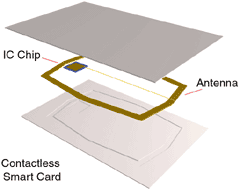
\includegraphics[scale=0.5]{card}
  	\caption{Contactless Smart Card}
  \end{center}
\end{figure}

\begin{figure}[H]
 \begin{center}
	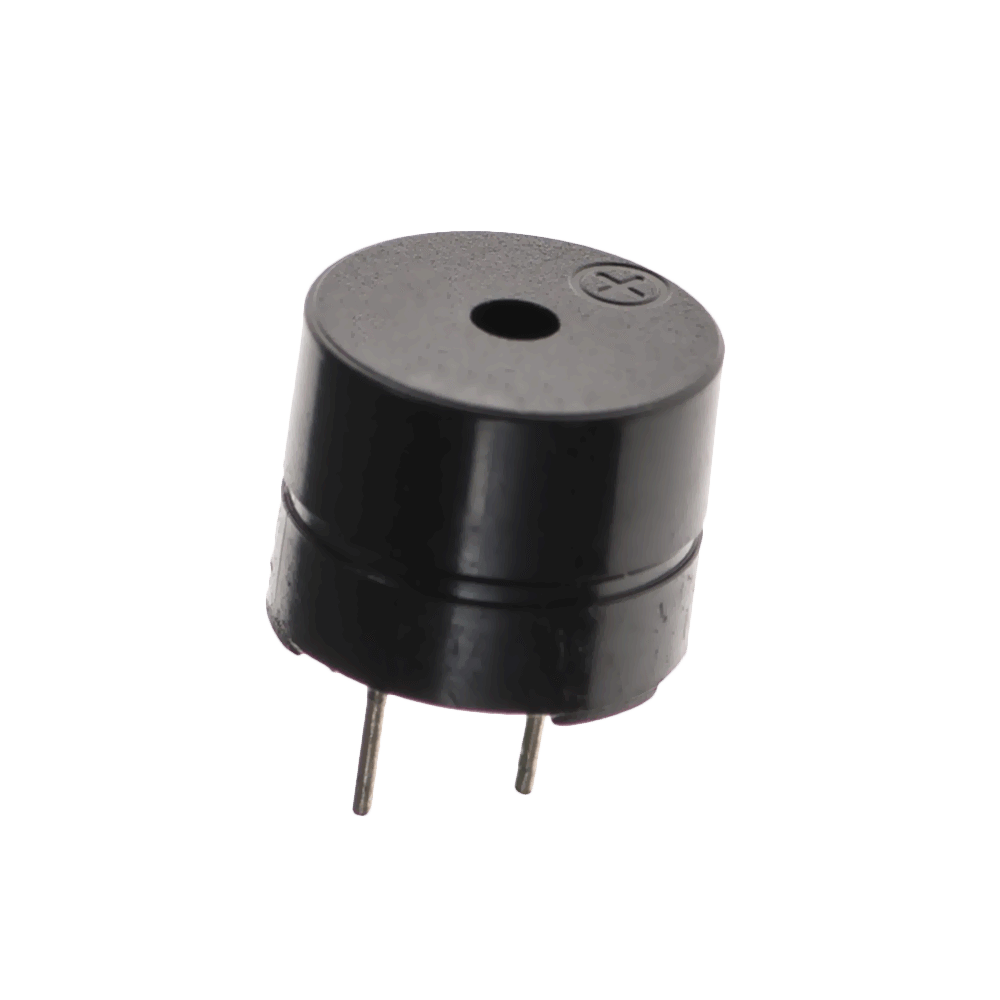
\includegraphics[scale=0.1]{buzzer}
  	\caption{Typical Buzzer}
  \end{center}
\end{figure}


\newpage
\section{Block Diagrams}
\begin{figure}[H]
 \begin{center}
	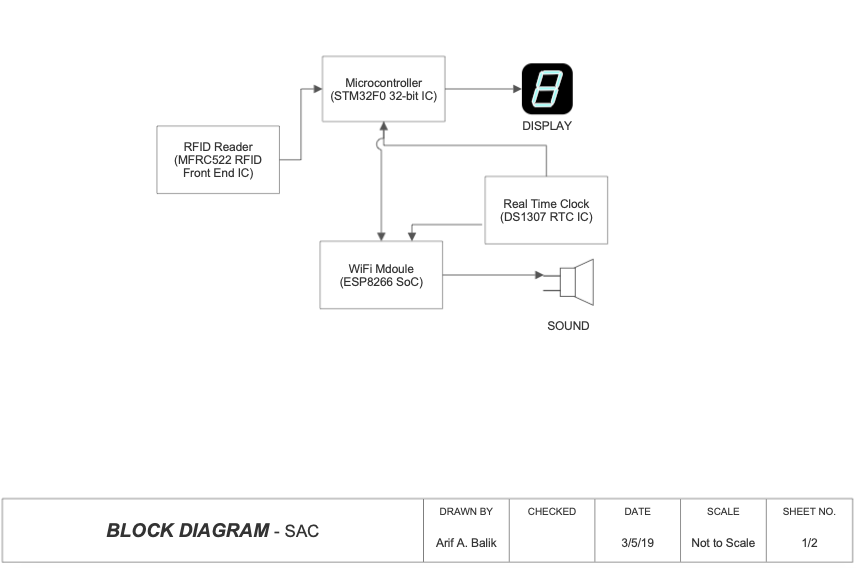
\includegraphics[scale=0.5]{bd2}
  	\caption{Overall Block Diagram for The Device}
  \end{center}
\end{figure}

\begin{figure}[H]
 \begin{center}
	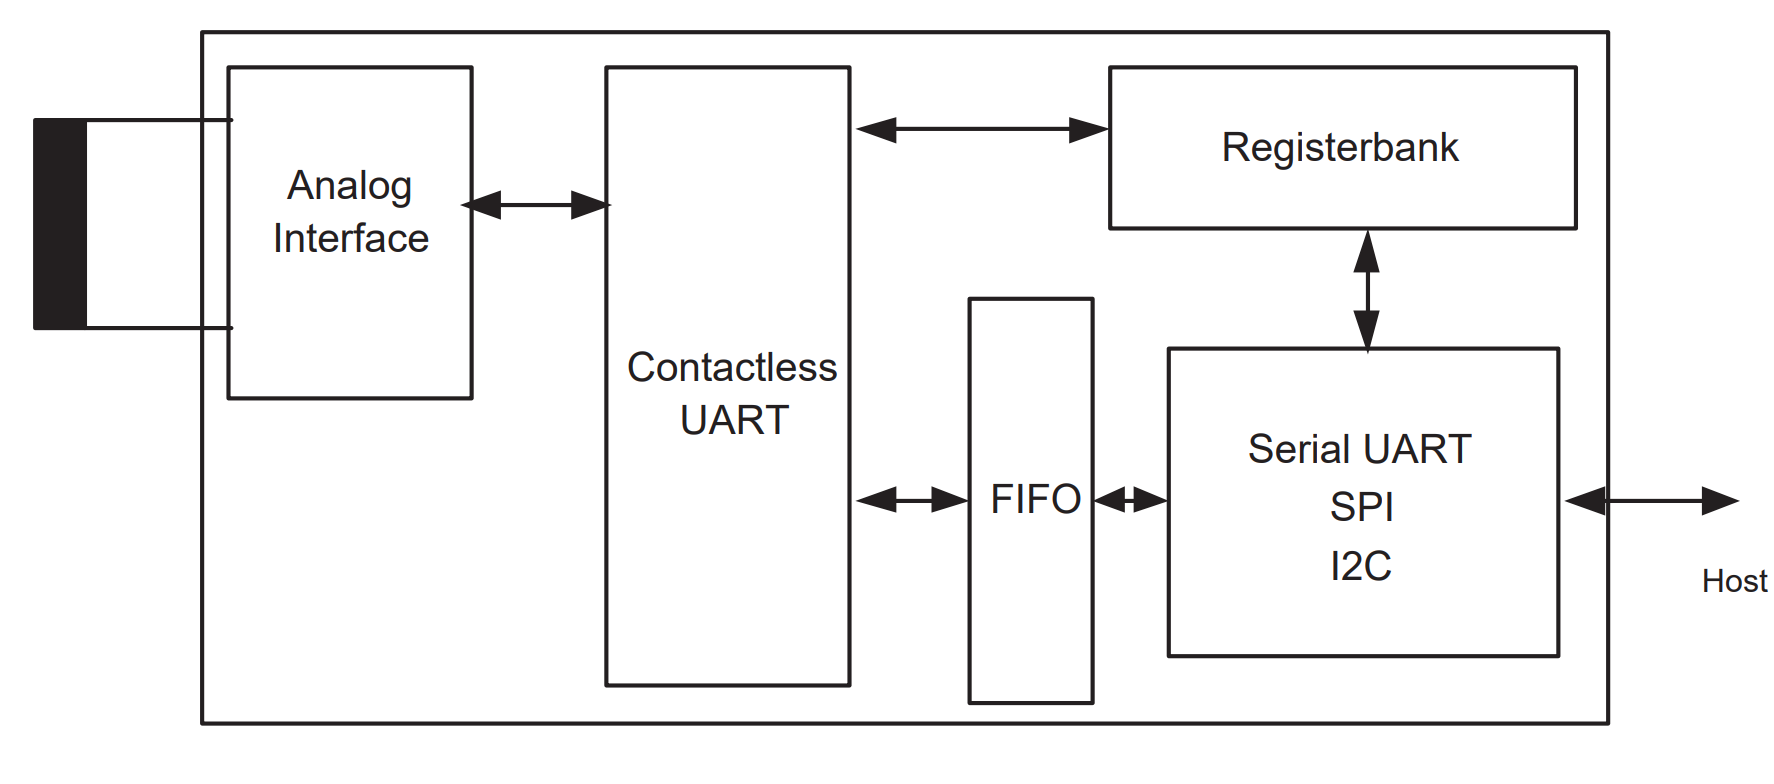
\includegraphics[scale=0.3]{rc522}
  	\caption{Simplified MFRC522 IC Diagram}
  \end{center}
\end{figure}
\section{Use Cases}
The following use cases gives a general scenario on how student and instructor may interact with the project. If reader seeks more detailed information, please check functional requirements and system features. 
\begin{figure}[H]
 \begin{center}
	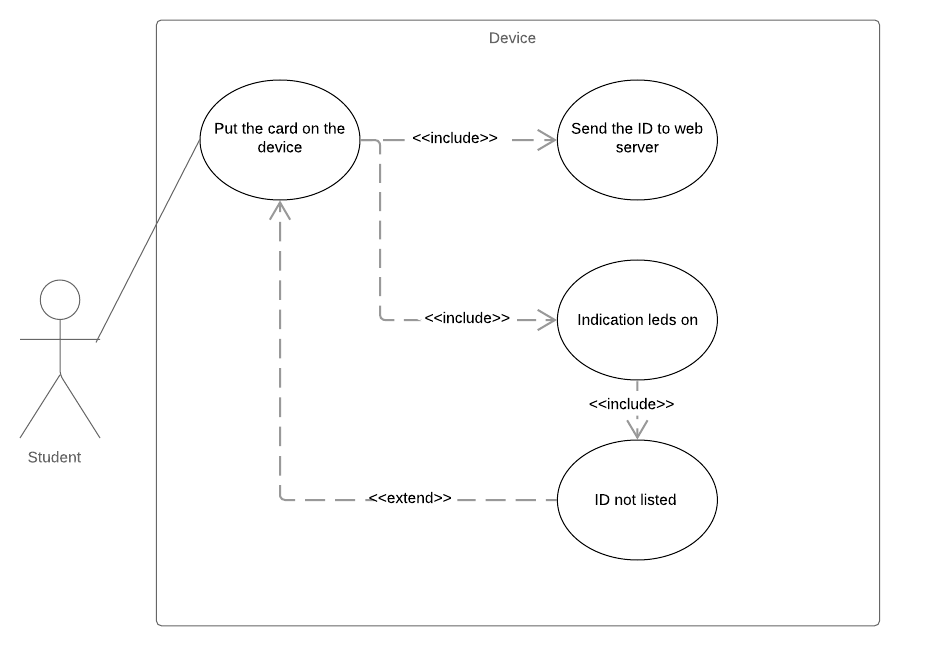
\includegraphics[scale=0.5]{student}
  	\caption{Student and Device Interaction}
  \end{center}
\end{figure}


\begin{table}[H]
 \begin{center}
\captionof{table}{Scenario : Put the card on the device }
\begin{tabular}{|c|l|}
\hline
\textbf{Name}                 & Put the card on the device                                                                                                                                      \\ \hline
\textbf{Actors}               & Student                                                                                                                                                         \\ \hline
\textbf{Description}          & Student use the card to log in to the class                                                                                                                     \\ \hline
\textbf{Succesful Completion} & \begin{tabular}[c]{@{}l@{}}1. Device sends the ID to server\\ 2. Server looks for a match\\ 3. Server returns success\\ 4. Indication LEDs turn on\end{tabular} \\ \hline
\textbf{Alternative}          & \begin{tabular}[c]{@{}l@{}}1. Device sends the ID to server\\ 2. Server looks for a match\\ 3. Server returns failure\\ 4. Indication LEDs turn on\end{tabular} \\ \hline
\textbf{Pre-condition}        & Student must have a valid RFID card                                                                                                                             \\ \hline
\textbf{Post-Conditions}      & None                                                                                                                                                            \\ \hline
\textbf{Assumptions}          & None                                                                                                                                                            \\ \hline
\end{tabular}
 \end{center}
\end{table}

\begin{figure}[H]
 \begin{center}
	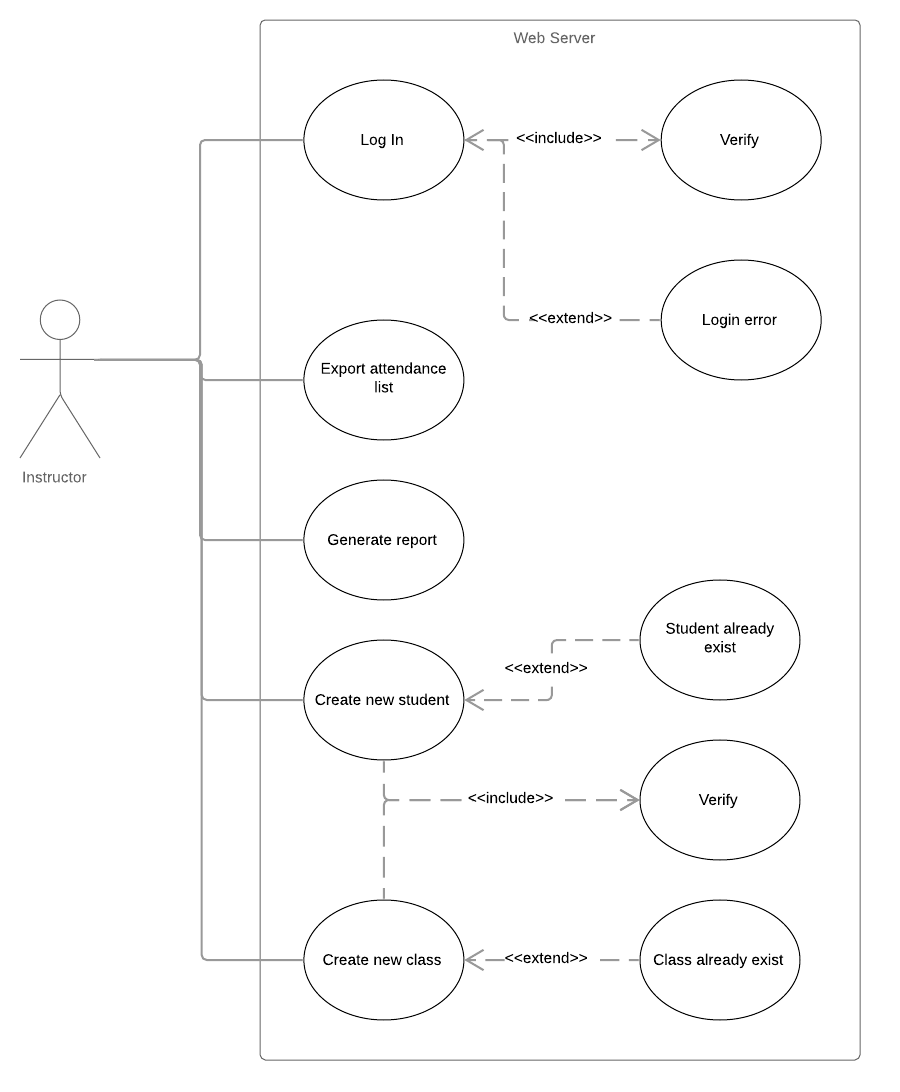
\includegraphics[scale=1]{instructor}
  	\caption{Instructor and Web Server Interaction}
  \end{center}
\end{figure}


\begin{table}[H]
\captionof{table}{Scenario : Log in }
\begin{tabular}{|c|l|}
\hline
\textbf{Name}                 & Log in                                                                                                                                                                                         \\ \hline
\textbf{Actors}               & Instructor                                                                                                                                                                                     \\ \hline
\textbf{Description}          & Instructor uses its id and password to log in the web server interface                                                                                                                         \\ \hline
\textbf{Succesful Completion} & \begin{tabular}[c]{@{}l@{}}1. Instructor types id and password\\ 2. Server looks for a match in the database\\ 3. Server finds a match\\ 4. Server starts the session\end{tabular}             \\ \hline
\textbf{Alternative}          & \begin{tabular}[c]{@{}l@{}}1. Instructor types id and password\\ 2. Server looks for a match in the database\\ 3. Server can not find a match\\ 4. Server prints an error message\end{tabular} \\ \hline
\textbf{Pre-condition}        & Instructor should have a computer and internet connection                                                                                                                                      \\ \hline
\textbf{Post-Conditions}      & None                                                                                                                                                                                           \\ \hline
\textbf{Assumptions}          & Instructor has id and password                                                                                                                                                                 \\ \hline
\end{tabular}
\end{table}

\begin{table}[H]
\captionof{table}{Scenario : Export Attendance List }
\begin{tabular}{|c|l|}
\hline
\textbf{Name}                 & Export Attendance List                                                                                                                                                                                                                                        \\ \hline
\textbf{Actors}               & Instructor                                                                                                                                                                                                                                                    \\ \hline
\textbf{Description}          & \begin{tabular}[c]{@{}l@{}}Instructor uses web server interface \\ to export a list of students who attended to class\end{tabular}                                                                                                                            \\ \hline
\textbf{Succesful Completion} & \begin{tabular}[c]{@{}l@{}}1. Instructor selects the class in the main menu\\ 2. Instructor uses the button located in the \\ main page named 'export'\\ 3. Server collects the data  and creates a .pdf file\\ 4. Instructor downloads the file\end{tabular} \\ \hline
\textbf{Alternative}          & None                                                                                                                                                                                                                                                          \\ \hline
\textbf{Pre-condition}        & Instructor should have a computer and internet connection                                                                                                                                                                                                     \\ \hline
\textbf{Post-Conditions}      & None                                                                                                                                                                                                                                                          \\ \hline
\textbf{Assumptions}          & Instructor is logged in                                                                                                                                                                                                                                       \\ \hline
\end{tabular}
\end{table}

\begin{table}[H]
\captionof{table}{Scenario : Generate Report }
\begin{tabular}{|c|l|}
\hline
\textbf{Name}                 & Generate Report                                                                                                                                                                                                                                                                         \\ \hline
\textbf{Actors}               & Instructor                                                                                                                                                                                                                                                                              \\ \hline
\textbf{Description}          & \begin{tabular}[c]{@{}l@{}}Instructor uses web server interface \\ to generate statistics\end{tabular}                                                                                                                                                                                  \\ \hline
\textbf{Succesful Completion} & \begin{tabular}[c]{@{}l@{}}1. Instructor selects the class in the main menu\\ 2. Instructor uses the button located in the \\ main page named 'generate report'\\ 3. Server collects the data  and generates statistic as a .pdf file\\ 4. Instructor downloads the file\end{tabular}   \\ \hline
\textbf{Alternative}          & \begin{tabular}[c]{@{}l@{}}1. Instructor selects the class in the main menu\\ 2. Instructor uses the button located in the main \\ page named 'generate report\\ '3. Server can not find enough data to generate statistic as a .pdf file\\ 4. Server prints error message\end{tabular} \\ \hline
\textbf{Pre-condition}        & Instructor should have a computer and internet connection                                                                                                                                                                                                                               \\ \hline
\textbf{Post-Conditions}      & None                                                                                                                                                                                                                                                                                    \\ \hline
\textbf{Assumptions}          & Instructor is logged in                                                                                                                                                                                                                                                                 \\ \hline
\end{tabular}
\end{table}

\begin{table}[H]
\captionof{table}{Scenario : Create New Student }
\begin{tabular}{|c|l|}
\hline
\textbf{Name}                 & Create New Student                                                                                                                                                                                                                                                                                                                \\ \hline
\textbf{Actors}               & Instructor                                                                                                                                                                                                                                                                                                                        \\ \hline
\textbf{Description}          & \begin{tabular}[c]{@{}l@{}}Instructor uses web server interface \\ to add new student into system\end{tabular}                                                                                                                                                                                                                    \\ \hline
\textbf{Succesful Completion} & \begin{tabular}[c]{@{}l@{}}1. Instructor clicks 'add student' button in the main page\\ 2. Instructor fills the information required, such as name, student id,\\ card id, department and presses 'save' button.\\ 3. Server checks if student already exist\\ 4. Student dont exist, server records the data in DB\end{tabular}  \\ \hline
\textbf{Alternative}          & \begin{tabular}[c]{@{}l@{}}1. Instructor clicks 'add student' button in the main page\\ 2. Instructor fills the information required, such as name, student id,\\ card id, department and presses 'save' button.\\ 3. Server checks if student already exist\\ 4. Student already exist, server prints error message\end{tabular} \\ \hline
\textbf{Pre-condition}        & Instructor should have a computer and internet connection                                                                                                                                                                                                                                                                         \\ \hline
\textbf{Post-Conditions}      & None                                                                                                                                                                                                                                                                                                                              \\ \hline
\textbf{Assumptions}          & Instructor is logged in                                                                                                                                                                                                                                                                                                           \\ \hline
\end{tabular}
\end{table}

\begin{table}[H]
\captionof{table}{Scenario : Create New Class }
\begin{tabular}{|c|l|}
\hline
\textbf{Name}                 & Create New Class                                                                                                                                                                                                                                                                                                     \\ \hline
\textbf{Actors}               & Instructor                                                                                                                                                                                                                                                                                                           \\ \hline
\textbf{Description}          & \begin{tabular}[c]{@{}l@{}}Instructor uses web server interface \\ to add new class into system\end{tabular}                                                                                                                                                                                                         \\ \hline
\textbf{Succesful Completion} & \begin{tabular}[c]{@{}l@{}}1. Instructor clicks 'add class' button in the main page\\ 2. Instructor fills the information required, such as name, \\ department, students and presses 'save' button.\\ 3. Server checks if class already exist\\ 4. Class dont exist, server records the data in DB\end{tabular}     \\ \hline
\textbf{Alternative}          & \begin{tabular}[c]{@{}l@{}}1. Instructor clicks 'add class' button in the main page\\ 2. Instructor fills the information required, such as name, \\ department, students and presses 'save' button.\\ 3. Server checks if class already exist\\ 4. Class already exist, server prints an error message\end{tabular} \\ \hline
\textbf{Pre-condition}        & Instructor should have a computer and internet connection                                                                                                                                                                                                                                                            \\ \hline
\textbf{Post-Conditions}      & None                                                                                                                                                                                                                                                                                                                 \\ \hline
\textbf{Assumptions}          & Instructor is logged in                                                                                                                                                                                                                                                                                              \\ \hline
\end{tabular}
\end{table}


{\let\clearpage\relax\chapter{External Interface Requirements}}

\section{User Interfaces}

\begin{enumerate}[leftmargin=5\parindent, label=UI-\arabic*:]
  \item Web application shall allow user to generate reports using mouse alone.
  \item All features of web application shall be accessible trough one page after successful log in.
\end{enumerate}

\section{Hardware Interfaces}
\begin{enumerate}[leftmargin=5\parindent, label=HI-\arabic*:]
   \item Student shall be able to initiate the process of attendance using the device with their student cards alone.
   \item Device shall inform the student about the attendance process in case of either success or failure.
   \item Device shall warn the instructor before battery runs out.
\end{enumerate}

Also following figure shows general description of hardware of project.
\begin{figure}
 \begin{center}
	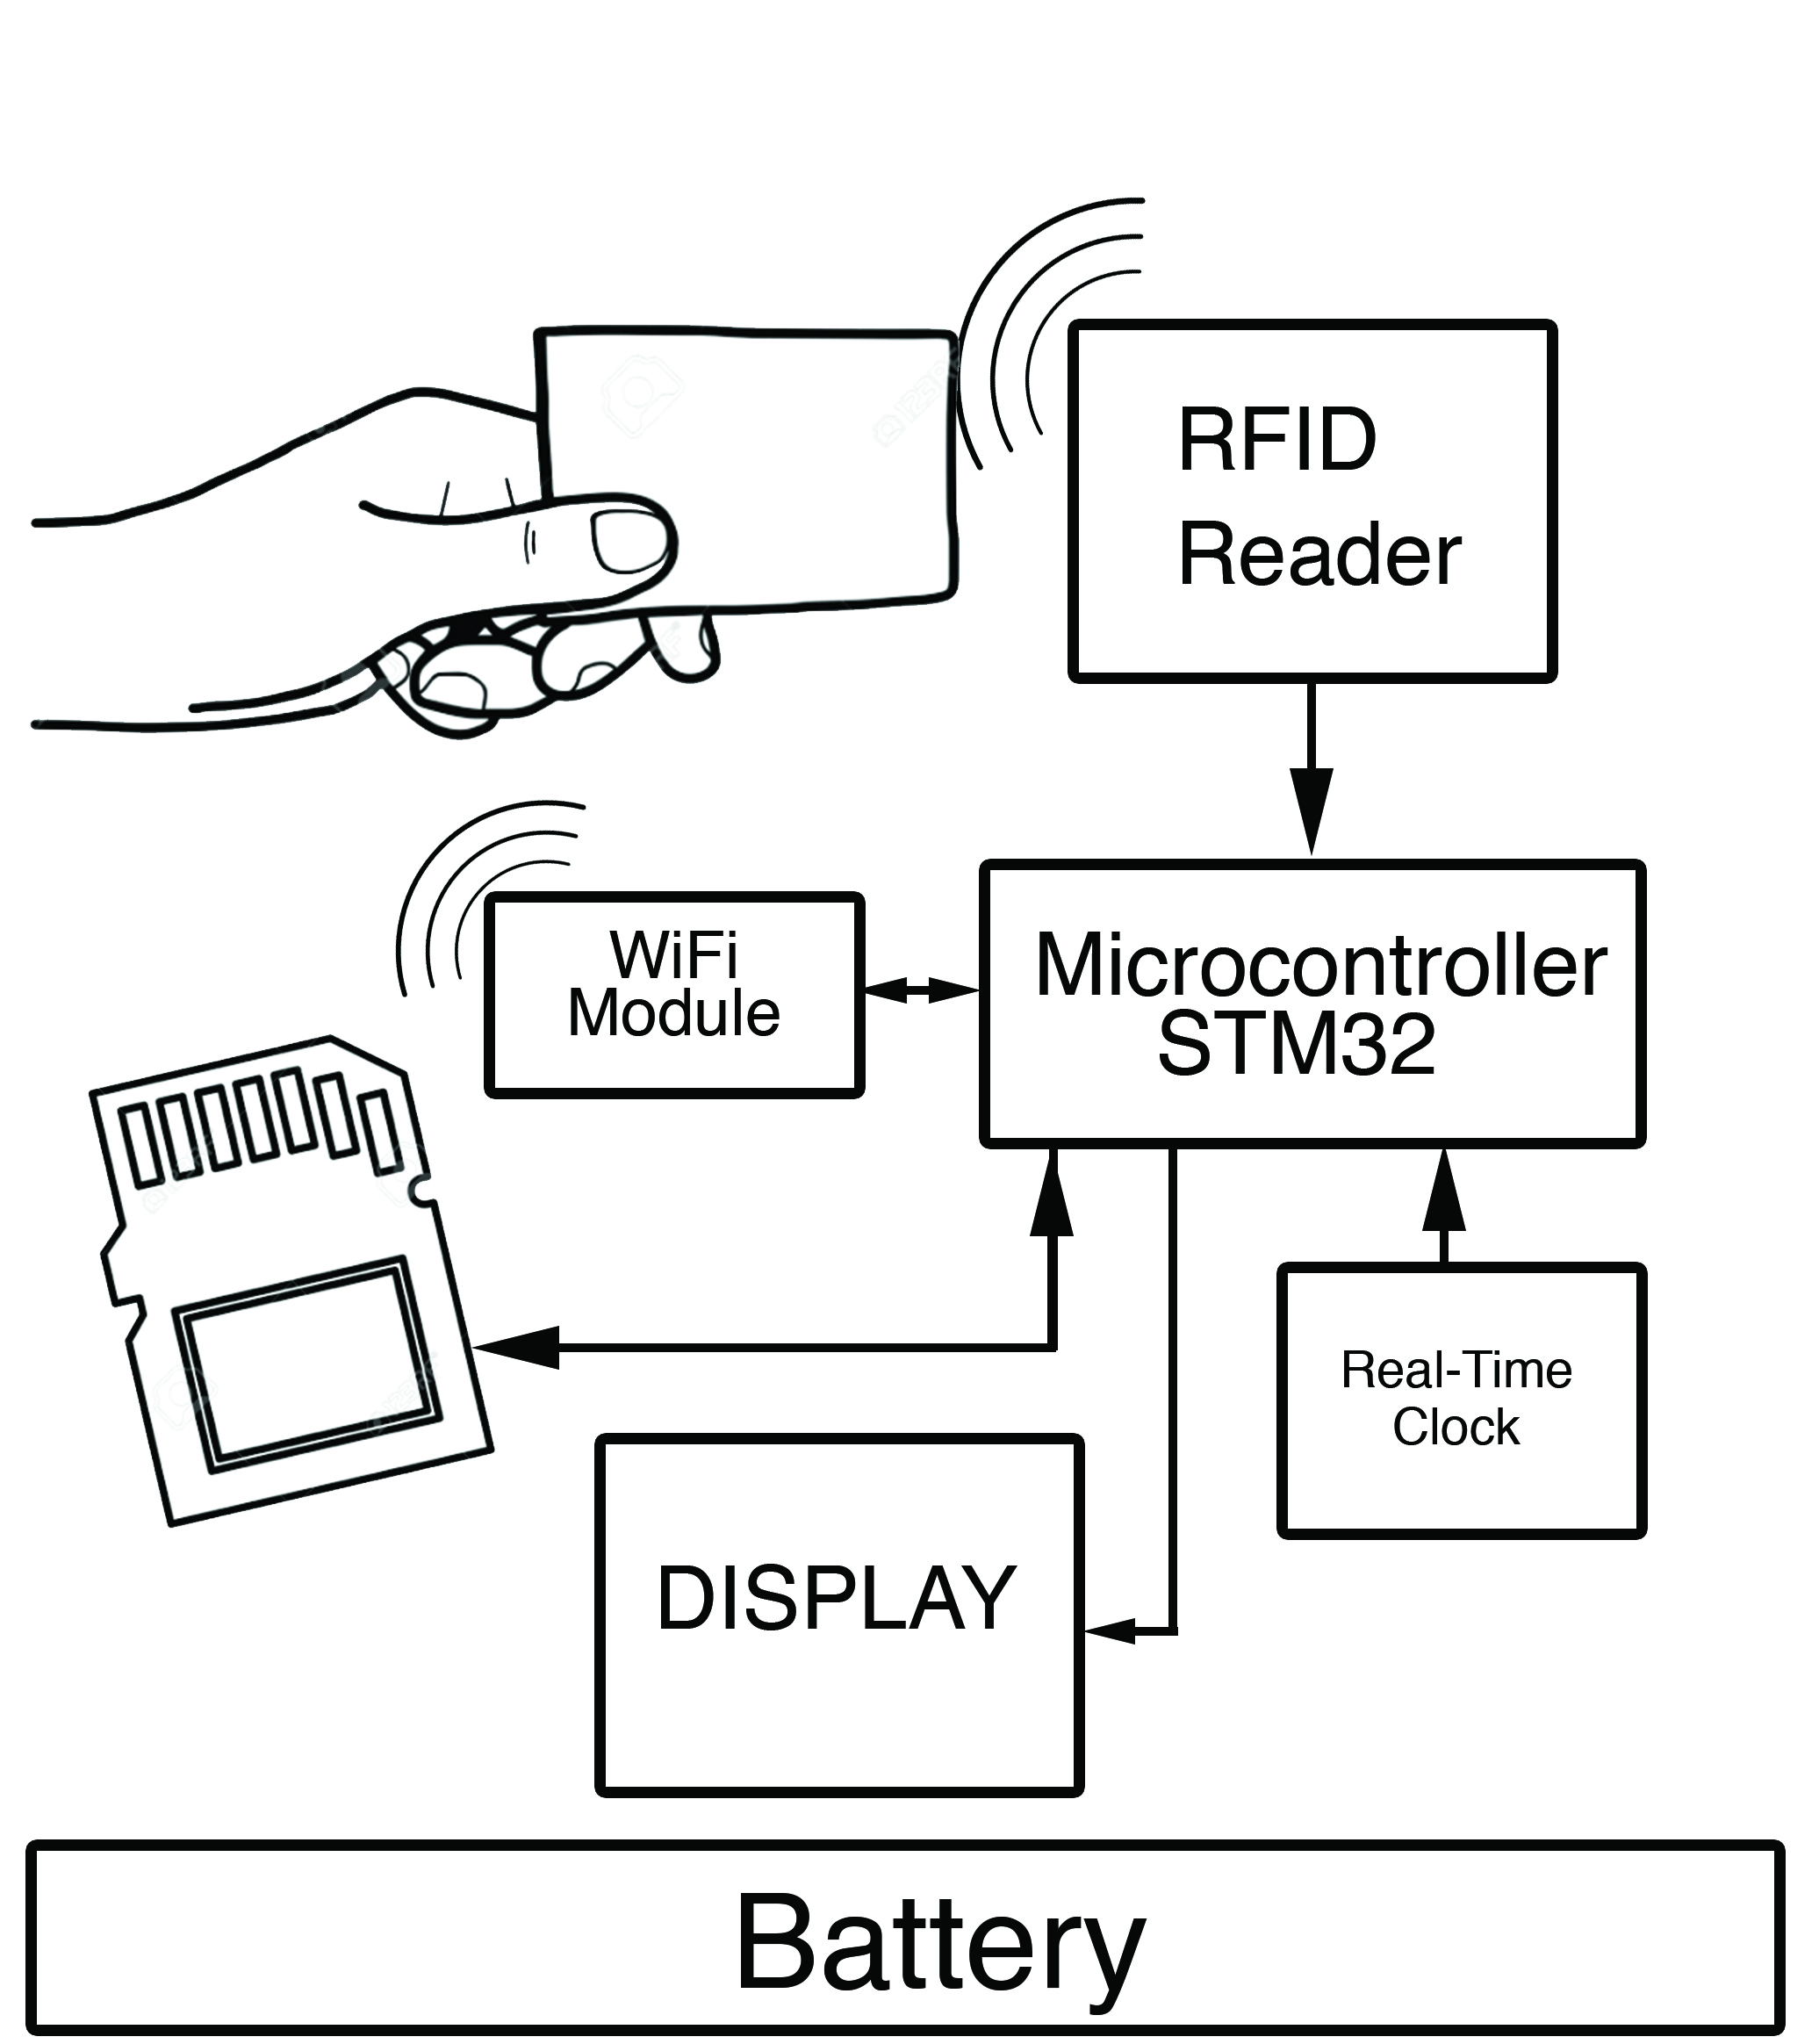
\includegraphics[width=80mm]{blockdiagram.jpg}
  	\caption{Internal modules of hardware}
  \end{center}
\end{figure}



\section{Software Interfaces}

\begin{enumerate}[leftmargin=5\parindent, label=SI-\arabic*:]
   \item Web Server
   	\begin{enumerate}[leftmargin=2\parindent, label=SI-1.\arabic*:]
	 	\item Web server shall communicate with the device
		\item Upon successful identification web server shall return success to the device
		\item Web server shall control every log in operation and print a related messages according to who logged in
		\item Web server shall handle every document to be created
		\item Web server shall store every process on the MySQL DB and inform the user about status of process
	\end{enumerate}
    \item Database - The system shall communicate with the database for following operations:
   	\begin{enumerate}[leftmargin=2\parindent, label=SI-2.\arabic*:]
	 	\item For every log in operation, checking whether user exists or not, and password is correct.
		\item To store attendance information real time.
		\item To add, delete or edit students, classes and users
		\item To generate reports
	\end{enumerate}
     \item Device
   	\begin{enumerate}[leftmargin=2\parindent, label=SI-3.\arabic*:]
	 	\item Device shall communicate with the web server
		\item Device shall send every RFID card it detects along with other informations as the following JSON format
			
			\begin{lstlisting}[frame=tlrb]
{
"Date": "13.04.2019 12:20:48 ",
"ID": 18383400,
"Key": 12345677890
}
			\end{lstlisting}
		\item Device shall listen server after sending any data, to inform student whether operation is successful or not.
	\end{enumerate}
\end{enumerate}

\begin{figure}[H]
 \begin{center}
	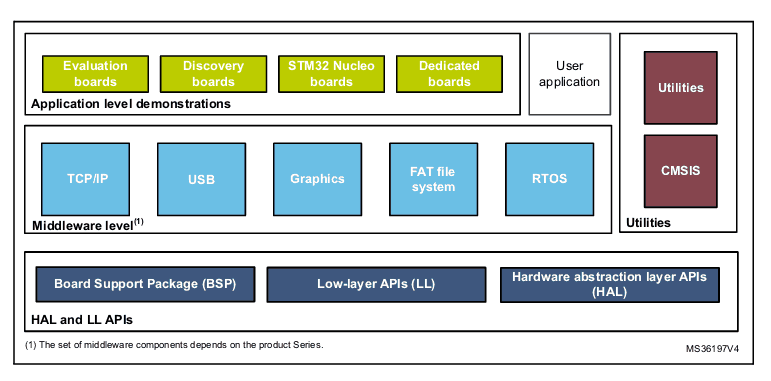
\includegraphics[scale=0.5]{cube}
  	\caption{Software layers for microcontroller}
  \end{center}
\end{figure}


\section{Communications Interfaces}
\begin{enumerate}[leftmargin=5\parindent, label=UI-\arabic*:]
  \item Web application shall send monthly reports automatically through email.
  \item Web application shall send an email for every revision or update on the software or terms.
\end{enumerate}

\chapter{Appendix}
\section{Appendix A: To Be Determined List}
\begin{itemize}
  \item How to communicate bidirectionally
  \item Solve the problem when student has courses which are overlapping
  \item Test the DB structre
\end{itemize}
\begin{figure}[H]
 \begin{center}
	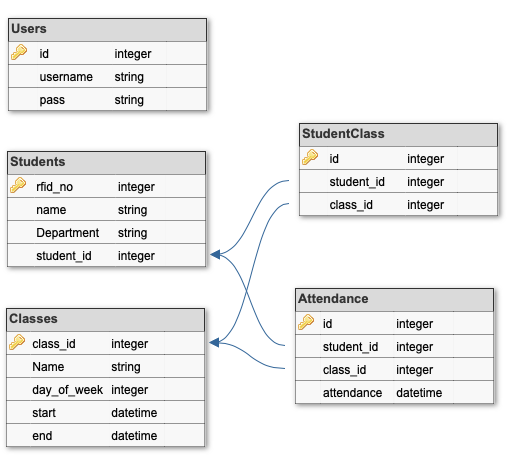
\includegraphics[scale=0.5]{db.png}
  	\caption{DB Structure}
  \end{center}
\end{figure}
\section{Appendix B: Lists}
\listoffigures
\listoftables




\end{document}
